\usetikzlibrary{calc}
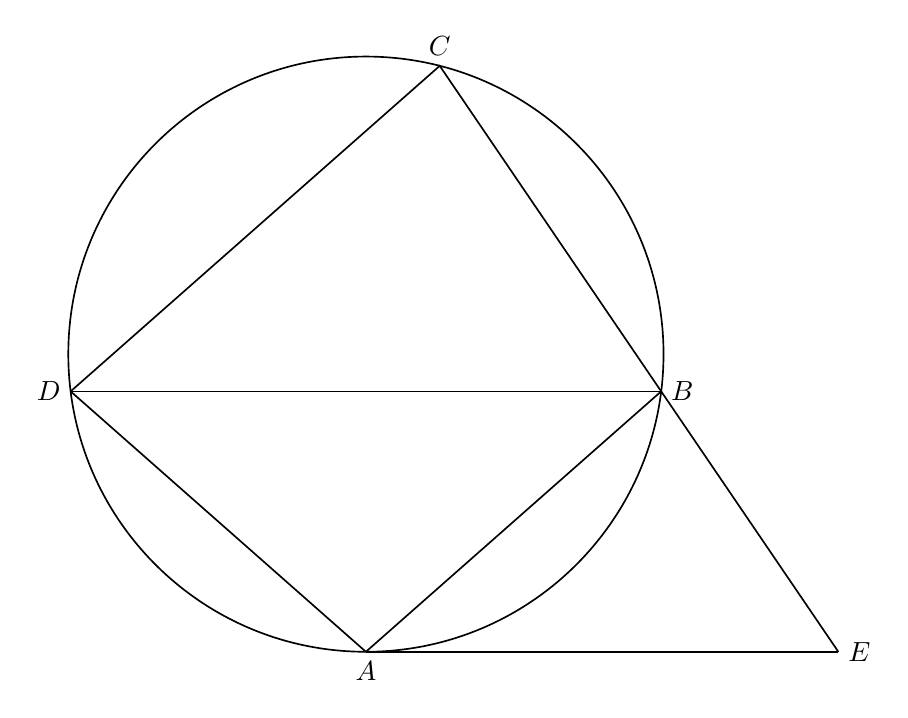
\begin{tikzpicture}[x=1cm,y=1cm,line width=.6pt,font=\normalsize]
\coordinate (O) at (5.2500,4.9796);
\coordinate (A) at (5.2500,1.2000);
\coordinate (B) at (9.0000,4.5072);
\coordinate (C) at (6.1875,8.6412);
\coordinate (D) at (1.5000,4.5072);
\coordinate (E) at (11.2500,1.2000);
\draw (O) circle[radius=3.7796cm];
\draw (D)--(C)--(E);
\draw (A)--(B);
\draw (A)--(D);
\draw (D)--(B);
\draw (A)--(E);
\node[above] at (C) {$C$};
\node[left] at (D) {$D$};
\node[right] at (B) {$B$};
\node[below] at (A) {$A$};
\node[right] at (E) {$E$};
\end{tikzpicture}
